\section{Introduction}
The main goal of this laboratory assignment is to explore different circuit analysis methods and to compare the results obtained with the results given by the \textit{Ngspice} simulation. For the theoretical analysis, the circuit will be analysed using mesh and nodal methods (both result from the Kirchoff's Laws) -  and the equations resulting from these methods will be solved using \textit{Octave}. On the other hand, the circuit simulation will be made, as said above, with \textit{Ngspice}. The analysed circuit can be seen in Fig. \ref{fig:esquema}.

\begin{figure}[h]
    \centering
    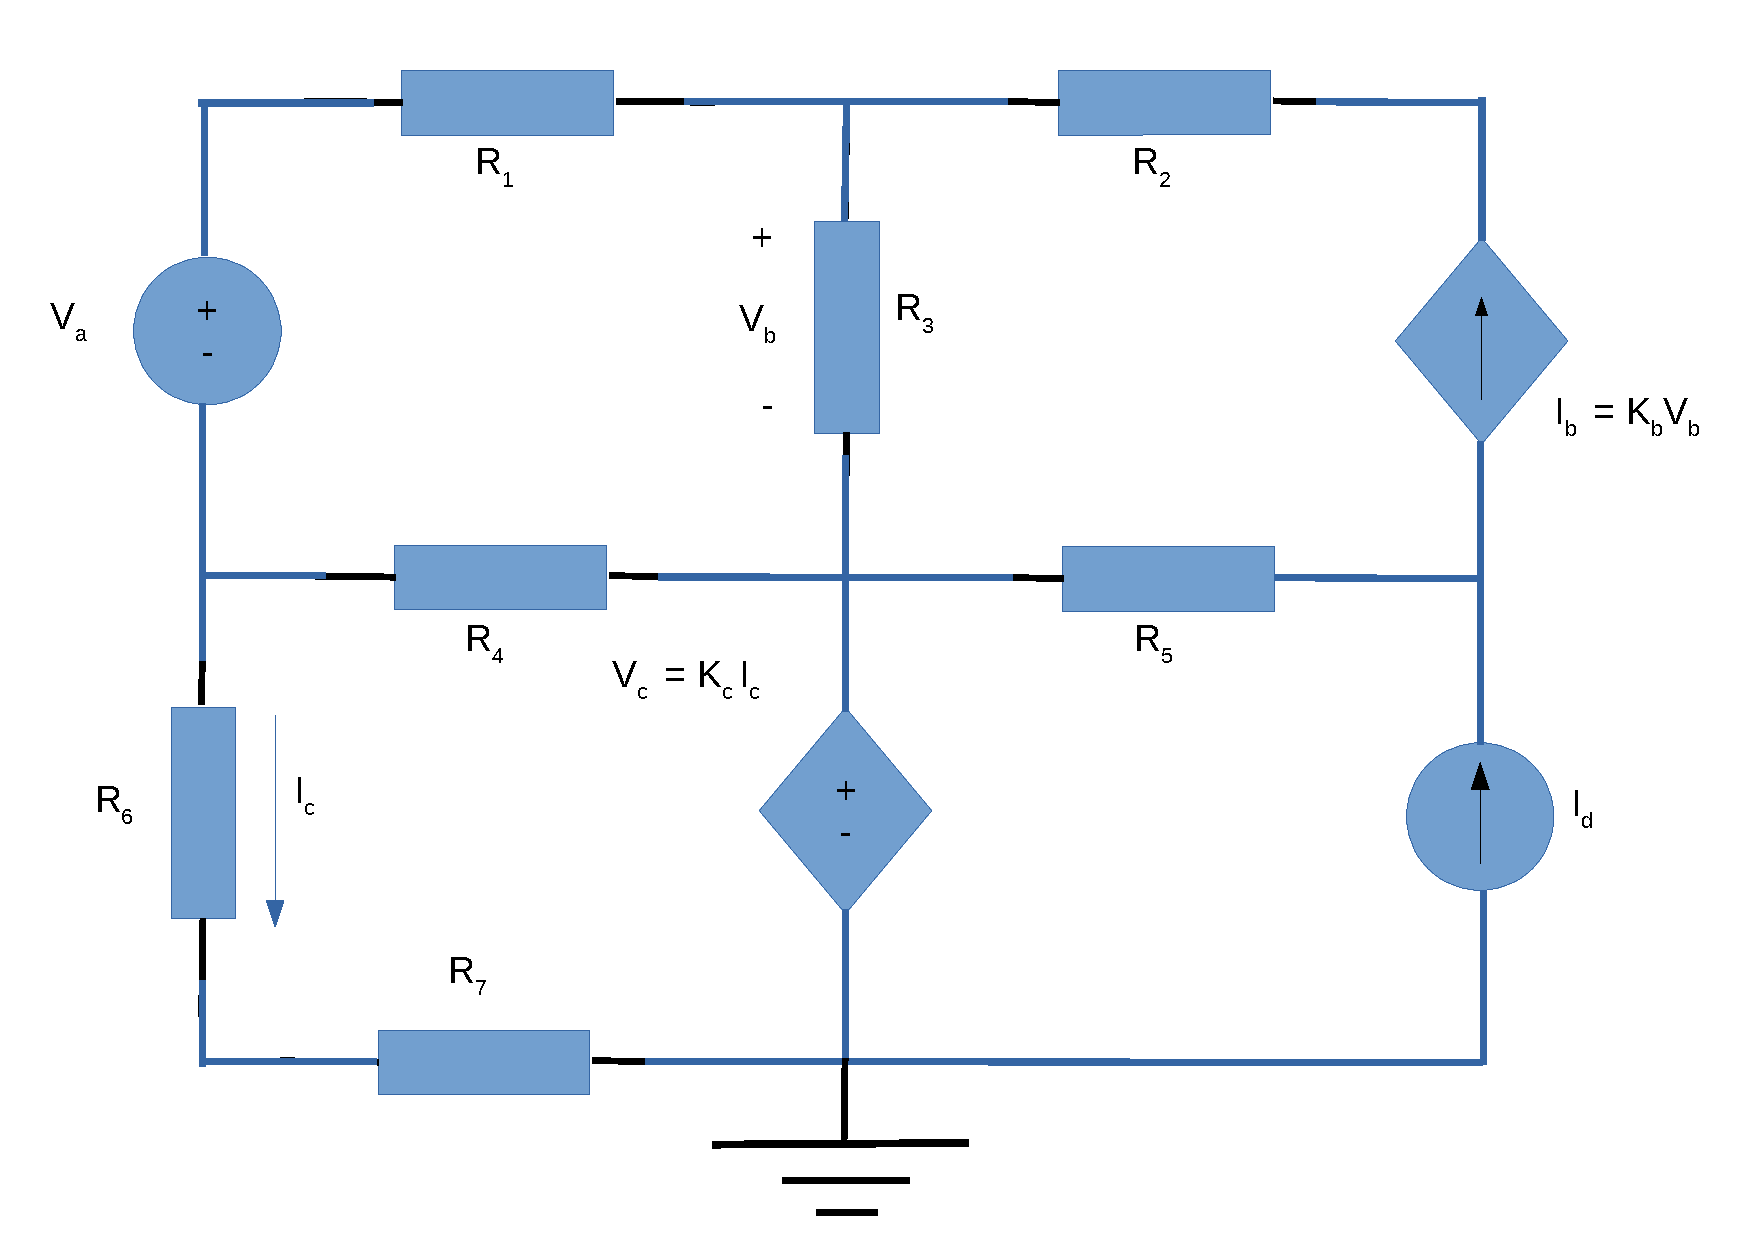
\includegraphics[width = 0.7\linewidth]{esquema.pdf}
        \caption{\textit{Circuit analysed. It consists, essentially, in a circuit with 4 essential meshes, 8 nodes and 11 branches (in which we count 7 resistors, 2 voltage sources - one of them controlled by the current $I_C$ - and 2 current sources - one independent and one dependent, controlled by the voltage $V_b$ as it can be seen in the figure. The labels used in this figure will be used throughout this report.}}
    \label{fig:esquema}
\end{figure}

As a starting point to solve this circuit, some values of the symbolic variables presented in Fig. \ref{fig:esquema} were given and are presented in Table \ref{tab:initial_values}:

\begin{table}[H]
    \begin{minipage}{.5\textwidth}
      \centering
      \begin{tabular}{c|c}
        \hline
        \multicolumn{2}{c}{Resistors [$k\Omega$]}  \\
        \hline
        $R_1$ & 1.03994439216 \\
        $R_2$ & 2.07923431764 \\
        $R_3$ & 3.06168544529 \\
        $R_4$ & 4.09516986362 \\
        $R_5$ & 3.00136467001 \\
        $R_6$ & 2.03324628446 \\
        $R_7$ & 1.02216788331
      \end{tabular}
    \end{minipage}
    \begin{minipage}{.5\textwidth}
      \centering
      \begin{tabular}{c|c}
        \hline
        \multicolumn{2}{c}{Currents [$mA$]}  \\
        \hline
        $I_d$ & 1.01674167773 \\
        \hline
        \hline
        \multicolumn{2}{c}{Voltages [$V$]}  \\
        \hline
        $V_a$ & 5.03847501972 \\
        \hline
        \hline
        \multicolumn{2}{c}{Dependent sources constants}  \\
        \hline
        $K_b$ & 7.01505323139 $mS$ \\
        $K_c$ & 8.37372457746 $k\Omega$
      \end{tabular}
    \end{minipage}
    \caption{Summary table with all the known values at the starting point}
    \label{tab:initial_values}
\end{table}